\section{What is Serverless Computing?}
\label{sec:serverless-computing}

\begin{figure}
  \begin{center}
    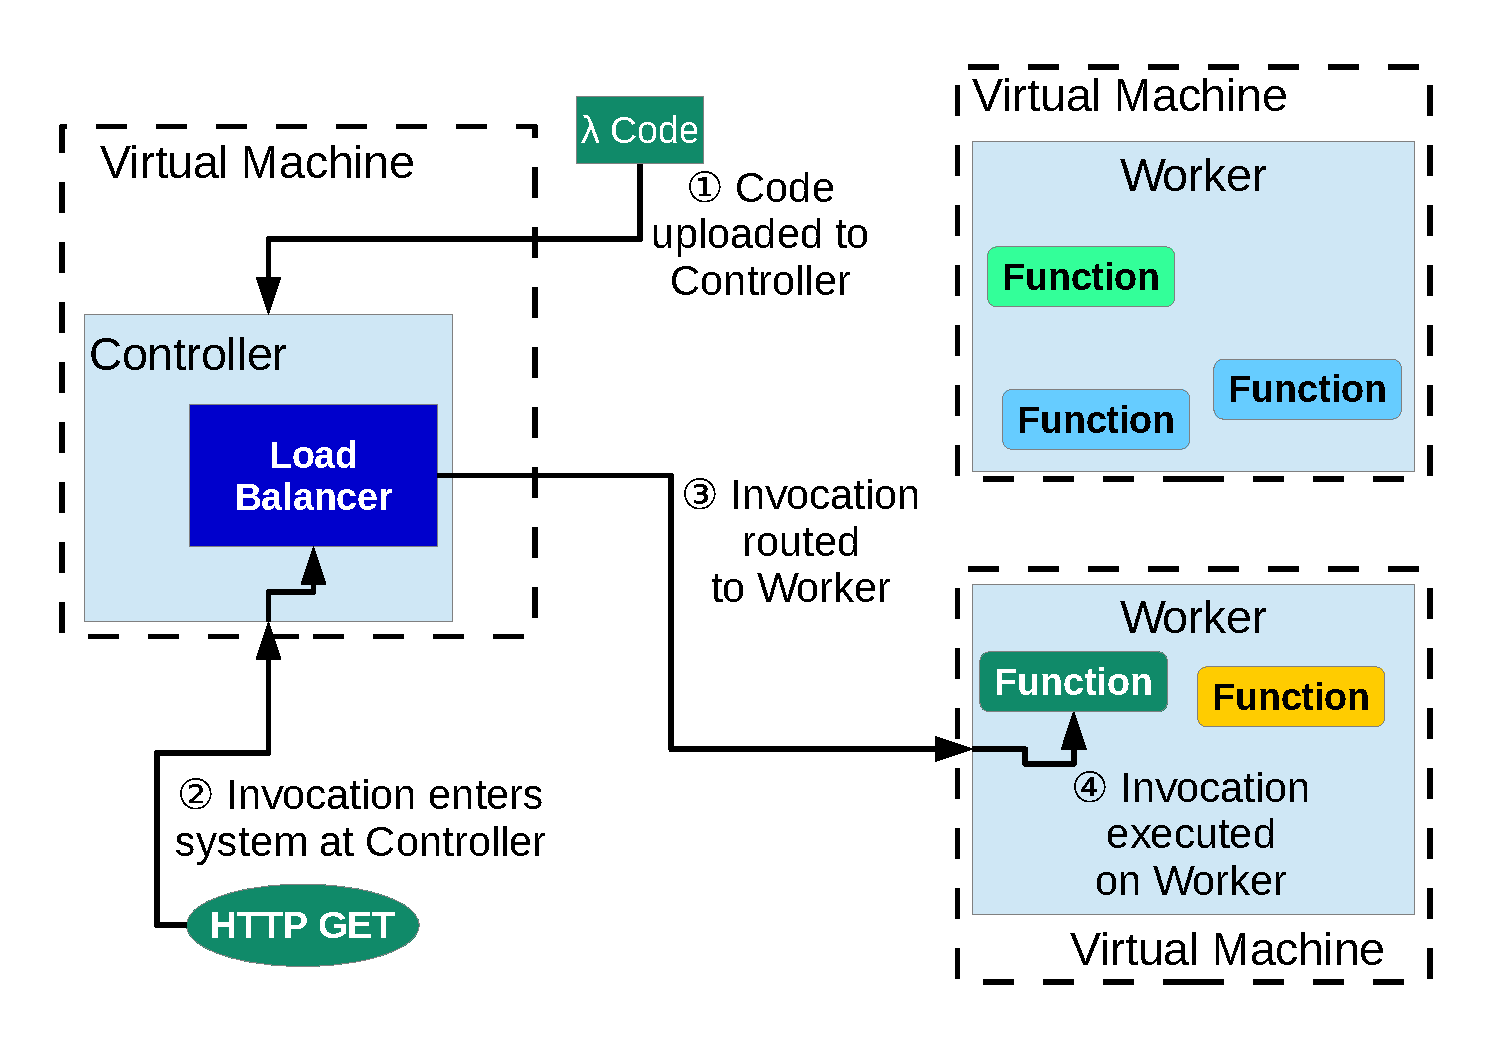
\includegraphics[width=.9\columnwidth]{./figures/sys-diag.pdf}
  \caption{A common architecture for serverless control planes. 
          A controller distributes invocations to workers who run them inside containers.}
  \label{fig:serverless-arch}
\end{center}
\end{figure}

% Continuing the container abstraction to its most extreme conclusion, we get a leap to \textit{serverless computing} often called Function-as-a-Service (FaaS).
Serverless computing presents a departure from previous iterations of cloud computing architectures.
Users can run arbitrary applications without concern for how or where it is ultimately run.
FaaS control planes operate as a complex distributed system, operating from the lowest levels of OS abstractions to the highest levels of cloud system designs.

All such control planes work similarly and follow the generic architecture shown in Figure~\ref{fig:serverless-arch}.
Users upload their \textit{source code} \circled{1} such as those in Figures~\ref{fig:python-lambda-example} and~\ref{fig:javascript-lambda-example} to the cloud provider to create a \textbf{function}, and such functions can be chained together inside the provider's system to form a larger \textbf{application}.
When the code is \textbf{invoked} (e.g. an HTTP request is made \circled{2}), the provider routes it to a worker \circled{3}, creates a sandbox for it and executes the function \circled{4}, passing in any custom parameters.
This sandbox must provide isolation, both covering both resource and security, ensuring that hogs or malicious actors do not interfere with co-located executions.
Often, this sandbox utilizes existing technologies such as Docker~\cite{docker-main} or VMs.
The major cloud computing providers have all created offerings, Amazon Lambda~\cite{lambda}, Google Cloud Functions~\cite{gcp-functions}, Azure Functions~\cite{azure-functions}, alternative providers such as IBM~\cite{openwhisk} and Alibaba~\cite{alibaba-compute} have joined in, and even non-commercial open-sourced control planes exist~\cite{hendrickson2016serverless,openfaas}.

\definecolor{deepblue}{rgb}{0,0,0.5}
\definecolor{deepred}{rgb}{0.6,0,0}
\definecolor{deepgreen}{rgb}{0,0.5,0}
% Python style for highlighting
\lstdefinelanguage{python}{
  keywords={self, import, as, def},
  morecomment=[l]{#},
  morecomment=[s]{"""}{"""},
  morestring=[b]',
  morestring=[b]",
  ndkeywords={self, import, as, def},
  keywordstyle=\color{blue}\bfseries,
  ndkeywordstyle=\color{darkgray}\bfseries,
  identifierstyle=\color{black},
  commentstyle=\color{purple}\ttfamily,
  stringstyle=\color{deepgreen}\ttfamily,
  sensitive=true
}
% \newcommand\pythonstyle{\lstset{
% language=python,
% % basicstyle=\ttm,
% morekeywords={self, import, as, def},              % Add keywords here
% keywordstyle=\ttb\color{deepblue},
% emph={MyClass,__init__},          % Custom highlighting
% emphstyle=\ttb\color{deepred},    % Custom highlighting style
% stringstyle=\color{deepgreen},
% morecomment=[l]{#},
% morecomment=[s]{"""}{"""},
% morestring=[b]',
% morestring=[b]",
% frame=single,                         % Any extra options here
% showstringspaces=false,
% basicstyle=\footnotesize\sffamily,
% columns=fullflexible,
% numbers=left,
% backgroundcolor=\color{lightgray},
% }}
% % Python environment
% \lstnewenvironment{python}[1][]
% {
% \pythonstyle
% \lstset{#1}
% }
% {}
\begin{figure}
  \begin{lstlisting}[language=python, numbers=left, frame=single, columns=fullflexible, label={lst:python-lambda-example}, basicstyle=\small]
# Initialization code 
import numpy as np 
import tensorflow as tf
  
m = download_model("http://model_serve/img_classify.pb")
session = create_tensorflow_graph(m) 
  
def lambda_handler(event, context):
    # This is called on every function invocation 
    picture = event["data"]
    prediction_output = run_inference_on_image(picture) 
    return prediction_output 
\end{lstlisting}
     \caption{A classic serverless function: simple Python code performing ML inference on image data. 
              In this example library and model initialization are done before execution starts.}
     \label{fig:python-lambda-example}
\end{figure}

\definecolor{lightgray}{rgb}{.9,.9,.9}
\definecolor{darkgray}{rgb}{.4,.4,.4}
\definecolor{purple}{rgb}{0.65, 0.12, 0.82}
\lstdefinelanguage{JavaScript}{
  keywords={break, case, catch, continue, debugger, default, delete, do, else, finally, for, function, if, in, instanceof, new, return, switch, this, throw, try, typeof, var, void, while, with},
  morecomment=[l]{//},
  morecomment=[s]{/*}{*/},
  morestring=[b]',
  morestring=[b]",
  ndkeywords={class, export, boolean, throw, implements, import, this},
  keywordstyle=\color{blue}\bfseries,
  ndkeywordstyle=\color{darkgray}\bfseries,
  identifierstyle=\color{black},
  commentstyle=\color{purple}\ttfamily,
  stringstyle=\color{red}\ttfamily,
  sensitive=true
}
\lstset{
   language=JavaScript,
   backgroundcolor=\color{white},
   extendedchars=true,
   basicstyle=\footnotesize\ttfamily,
   showstringspaces=false,
   showspaces=false,
   numbers=left,
   numberstyle=\footnotesize,
   numbersep=9pt,
   tabsize=2,
   breaklines=true,
   showtabs=false,
   captionpos=b
}
\begin{figure}
  \begin{lstlisting}[language=JavaScript, numbers=left, frame=single, basicstyle=\small, columns=fullflexible]
const doc = require("dynamodb-doc");    
const dynamo = new doc.DynamoDB();

exports.handler = (event, context, callback) => {
    const done = (err, res) => callback(null, {
        statusCode: err ? "400" : "200",
        body: err ? err.message : JSON.stringify(res),
        headers: {
          "Content-Type": "application/json",
        },
    });
    switch (event.httpMethod) {
        case "DELETE":
            dynamo.deleteItem(JSON.parse(event.body), done);
            break;
        case "GET":
            dynamo.scan({ TableName: event.queryParams.TableName }, done);
            break;
        case "POST":
            dynamo.putItem(JSON.parse(event.body), done);
            break;
        case "PUT":
            dynamo.updateItem(JSON.parse(event.body), done);
            break;
        default:
            done(new Error("Unsupported method `${event.httpMethod}'"));
    }};
     \end{lstlisting}
     \caption{Functions have varied tasks and implementation languages.
     This JavaScript function is designed to operate a microservice as part of a larger application.}
     \label{fig:javascript-lambda-example}
\end{figure}

\begin{comment}
  \begin{figure}
  \begin{lstlisting}[frame=single, basicstyle=\small, columns=fullflexible]
GET http://faas.com/img_recogn?input_bucket=9bcc64b9.png
  \end{lstlisting}
  \caption{Invoking a serverless function to perform image recognition. Small inputs may be passed directly, with large ones passed indirectly via storage.}
  \label{fig:lambda-invoke}
\end{figure}
\end{comment}


FaaS functions are extremely diverse, encouraged by platforms who want to make it easy to adapt code of any type.
% One of the  Figure~\ref{fig:python-lambda-example} is
An extremely common example is Figure~\ref{fig:javascript-lambda-example}, a microservice written in JavaScript that will operate as part of a larger application.
The other common language is Python, often used for ML inference functions like Figure~\ref{fig:python-lambda-example}.
Previously running applications like these would need VMs to host each piece, or managing a complex orchestration tool such as Kubernetes~\cite{kubernetes}.
The transition to FaaS also removes the need to manually scale how many instances of each service are running as user demand grows and shrinks.

In a change from the billing model for rented VMs, users are billed only for the time their code is executing, often in small millisecond-sized time slices.
Most providers set the cost to a formulation of the amount of memory used per time period~\cite{lambda-pricing}, roughly $\$1.66 \times 10^{-5}$ per GB/second.
Should the provider choose to keep that sandbox resident in memory to use for a future invocation, the user will not be charged nor be aware that it is happening, save for lower latency on future invocations.

%~\cite{lambda,gcp-functions,azure-functions,openwhisk,alibaba-compute,shahrad2020serverless,hendrickson2016serverless}


% Serverless computing is now being provided by all large public cloud providers and is an increasingly popular way to deploy applications on the cloud.  
%Amazon Lambda~\cite{aws-lambda}, Google Functions~\cite{google-functions}, and Azure Functions~\cite{azure-functions} are becoming an
% Functions as a Service (FaaS) can also be realized on private clouds and dedicated clusters using frameworks such as OpenWhisk~\cite{openwhisk}, OpenFaaS~\cite{openfaas},  OpenLambda~\cite{hendrickson2016serverless}, etc. 
% In this new cloud paradigm, users provide functions in languages such as Python, JavaScript, Go, Java, and others. 
% The functions are executed by the FaaS platform, greatly simplifying resource management for the application. 



% Need to explain how it all works. But first provide some context for why this is important.


%In order to provide FaaS, the way it is implemented by platforms, results in certain performance challenges.
%However, the execution of FaaS functions entails performance overheads that we must be cognizant of. 
%
%FaaS functions cannot assume that state will persist across invocations, and functions need to be self contained in terms of their dependencies. 
%

\subsection{Function Isolation}

Each function is run inside an isolated sandbox environment such as a Docker container~\cite{docker-main}, or a lightweight VM such as Firecracker~\cite{firecracker-nsdi20}. 
By encapsulating function state and any side effects, the virtual execution environment provides isolation among multiple functions, and also allows for concurrent invocations of the same function. 
Due to the overhead of starting a new virtual execution environment (i.e., container or VM), and initializing the function by importing libraries and other data dependencies, function execution thus incurs a significant \quotes{cold-start} penalty.
Table~\ref{tab:bg-workloads} shows the breakdown of initialization time (last column) vs. the total running time of different FaaS applications, and we can see that the initialization overhead can be as much as 80\% of the total running time. 
Thus, FaaS can result in significant performance (i.e., total function execution latency) overheads compared to conventional models of execution where applications can maintain application state between handling user requests and do not face the high initialization and cold-start overheads.



\begin{table}
  \centering
  \caption{FaaS workloads are highly diverse in their resource requirements and running times. The initialization time can be significant and is the cause of the cold-start overheads, and depends on the size of code and data dependencies.}
  \begin{tabular}{lrrr}
    \hline 
    Application & Memory size & Run time & Initialization time \\
    \hline
    ML Inference (CNN) & 512 MB & 6.5 s & 4.5 s \\
    Video Encoding & 500 MB & 56 s & 3 s \\
    Matrix Multiply & 256 MB & 2.5 s & 2.2 s \\
    Disk-bench (\texttt{dd})  & 256 MB & 2.2 s & 1.8 s \\
    % Image Manip & 300 MB & 9 s & 6 s \\
    Web-serving & 64 MB & 2.4 s & 2 s \\
    Floating Point & 128 MB & 2 s & 1.7 s \\
    \hline
  \end{tabular}
  % \vspace*{\myfigspace}
  \label{tab:bg-workloads}
  %\vspace*{\myfigspace}
\end{table}



% Replace two main techniques -> Only one technique. 
%Two main techniques are used to alleviate the cold-start penalty. 
% Once a container for a function is created and the function finishes execution, the container can be kept alive instead of immediately terminating it. 
% Subsequent invocations of the function can then \emph{reuse} the already running container.
% This \emph{keep-alive} mechanism can alleviate the cold-start overhead due to container launching (which can be $\sim 100$ ms). %Might be confusing, keep-alive also helps in other initialization.

% However, keep-alive is not a panacea for all FaaS latency problems. 
% Keeping a container alive consumes valuable computing resources on the servers. %, and reduces the number of functions that can be executed concurrently. 
% Specifically, a running container occupies memory, and \quotes{warm} containers being kept alive in anticipation of future function invocations can reduce the multiplexing and efficiency of the servers. 
% Thus, we develop keep-alive \emph{policies} that reduce the cold-start overhead while keeping the server utilization high.

% Designing general keep-alive policies is challenging due to the extreme heterogeneity in the different function popularities, resource requirements, and cold-start overheads.
% For instance, a recent analysis of FaaS workloads from Azure~\cite{shahrad_serverless_2020} shows that function inter-arrival times and memory sizes can vary by more than three orders of magnitude.
% This workload heterogeneity magnifies the performance vs. utilization trade off faced by keep-alive policies, as we shall describe in the next section. 
% Additionally, FaaS workloads also show a high temporal dynamism, which requires new approaches to resource provisioning and elastic scaling, which we also develop. 

\section{Virtualization for FaaS}
\label{sec:virtualization}


\subsection{Virtual Machines}

% Turtles all the way down.
% The public cloud is build on virtualized components.
% Compute providers have vast quantities of physical hardware and sell virtualized resources to customers~\cite{amazon-ec2, azure-compute, google-compute}.
% Rather than having to procure and 

To both prevent takeover of the physical hardware and ensure isolation between different users, cloud providers typically offer virtualized infrastructure~\cite{xen}.
Mimicking the stack in Figure~\ref{fig:vms}, user applications run inside a virtual machine and cannot directly access the hardware.
A hypervisor manages a set of virtual machines that have a private OS inside them.
Using hardware virtualization techniques, the provider's hypervisor interposes itself between guest and hardware, maintaining total control.
Memory is protected via virtual memory in the CPU, protected instructions are trapped to the hypervisor, and network and disk I/O interaction can be run through the hypervisor.
A major drawback is that users must install (duplicate) copies of OS's, libraries, and applications into each VM, and are responsible for maintenance of the guest OS.

% Basic outline of a Virtualization setup.
% Hypervisor, Mangagement software, various guests.
% hypervisor imposes as fake version of hardware for isolation.

\subsection{VM Resource Management}

% Boil 'em, mash 'em, stick 'em in a rack.
% Oodles of work in the maximizing resource use in area.
% From making them faster, reducing footprint, bin-packing, etc.
A number of works have sought to reduce the overhead from virtualization by techniques such as securely exposing hardware to guests~\cite{dong2008sr} or reducing layers of indirection~\cite{ben2010turtles}.
A number of optimizations to memory usage that reduce the footprint of VMs were outlined by~\cite{waldspurger2002memory}, which are still used in production hypervisors today.
Choosing where to place VMs, knowing that they may run for days or months, is critical to reduce fragmentation on hosts across provider datacenters.
Bin-packing studies have sought to minimize fragmentation~\cite{binpacking} by overcommitting resources even at the risk of violating capacity.
Even today, after much research in the area, providers see 20\%-40\% of unallocated resources~\cite{fuerst2022memory} that they seek ways to make use of.

\subsection{Containers}

% \begin{figure}
%   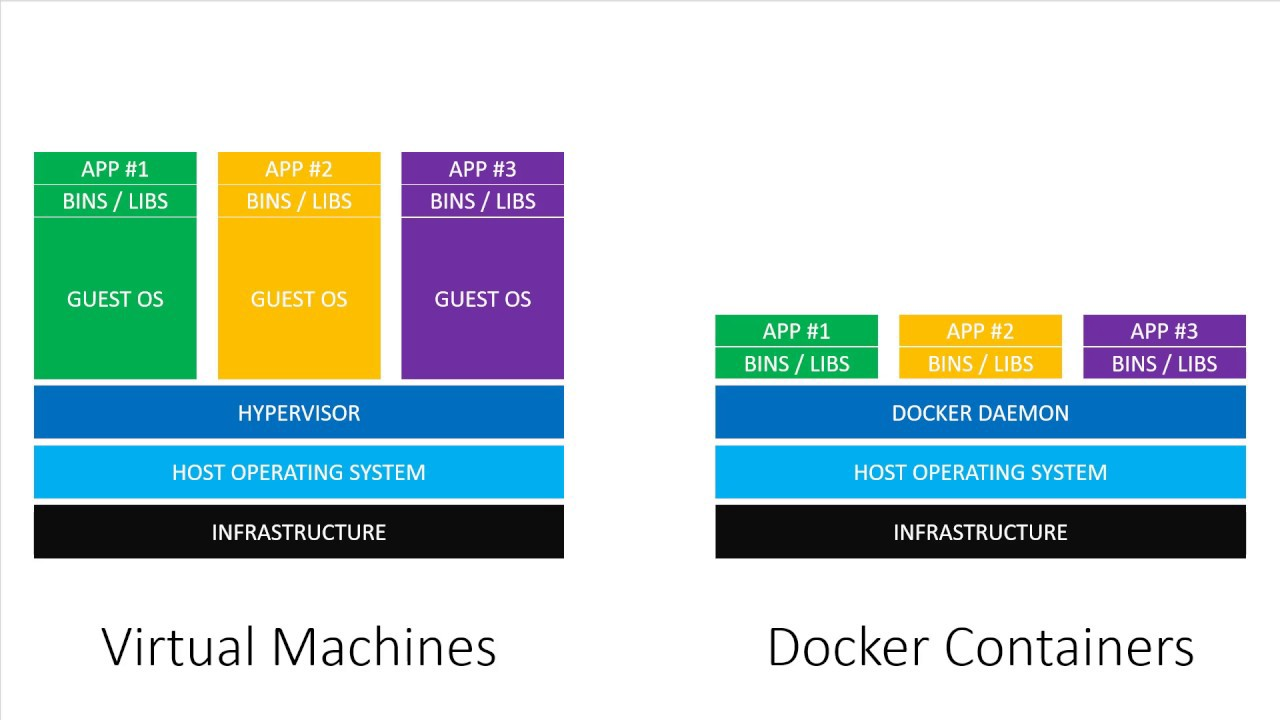
\includegraphics[width=\columnwidth]{figures/docker-vs-vms.png}
% \end{figure}

\begin{figure}
  \subfloat[Virtual Machines]{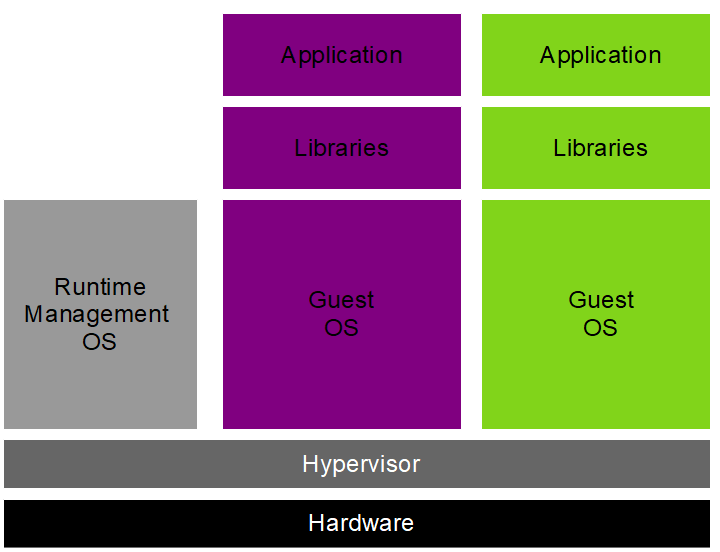
\includegraphics[width=0.5\textwidth]{serverless/figs/vms.png} \label{fig:vms}}
  \subfloat[Containers]{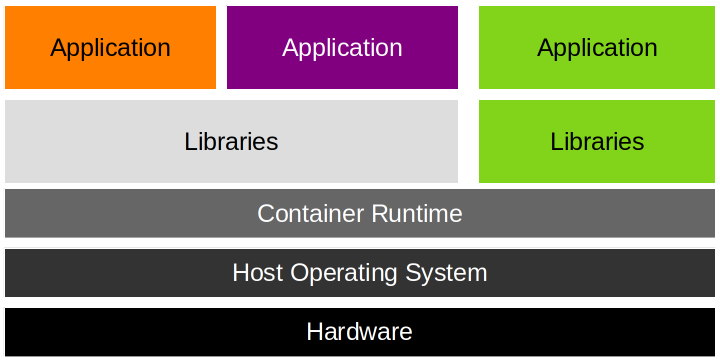
\includegraphics[width=0.5\textwidth]{serverless/figs/containers.png} \label{fig:docker}}
  \caption{Different layers of abstraction between hardware and kernel based virtualization.}
  \label{fig:docker-vs-vms}
\end{figure}

Enabling both improved process-level protections and a viable alternative to hardware virtualization, a new method of isolation was devised.
Kernel virtualization, built originally around Linux \textit{cgroups}, provides similar isolation and security guarantees to VMs.
A combination of kernel utilities enables limiting CPU, memory, and I/O usages, restricting views of the file system, blocking interaction with other processes, and more.
Popularized by various projects~\cite{oci,docker-main}, such \textit{containers} reimagined how cloud computing and applications could work.
Multiple applications could share the same operating system, and even libraries, safe from all interference from one another.
Developers could ship applications, complete with any dependencies, that ran securely, anytime, and anywhere.
Providers have begun offering services around these, tools like Kubernetes~\cite{kubernetes} orchestrate placement of containers onto hosts, removing the need for users to rent VMs at all.
